\chapter{FUNDAMENTALS OF A STEVE PROGRAM} \label{ch:pipeline_model}

This chapter describes the fundamentals parts of a Steve program: how it works,
how its structured, and what algorithms it relies on to process packets.
Before a programmer can begin writing a Steve program, they must understand
two important concepts: 

\begin{enumerate}
\item how a Steve program divides between data and control planes and
\item the \emph{packet processing pipeline} abstract model.
\end{enumerate}

\section{Structure of a Steve Program}

A Steve program is a list of declarations. These declarations describe
packet structure, decoders, flow tables, and event handlers.
These entities may be split into two categories:
entities which define data plane processing and
entities which define control plane logic. 
Figure \ref{fg:abstract_switch} demonstrates this divide.

\begin{figure}[ht]
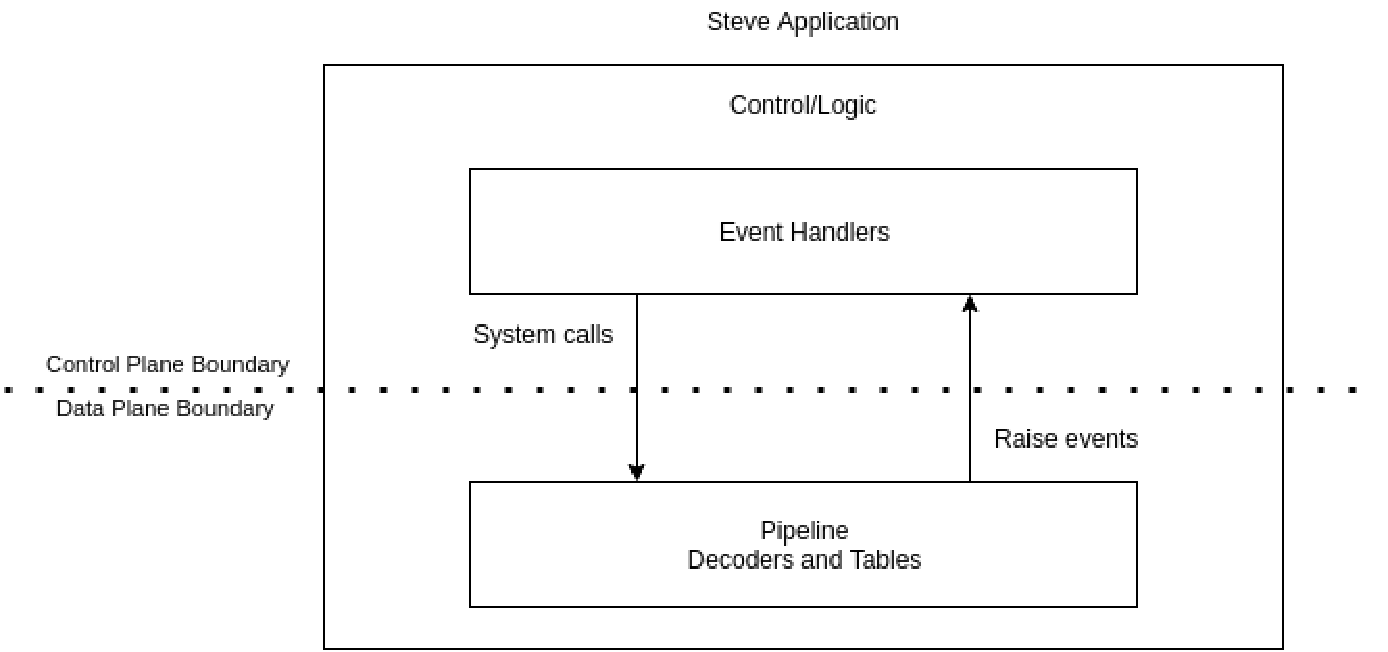
\includegraphics[width=\linewidth]{steve_model}
\caption{Steve program entities and how the split between control and
data planes. The data plane's pipeline raise events which are handled by event 
handlers on the control plane. Event handlers make system calls back to the
data plane to modify pipeline behavior or to re-enter special packets.}
\label{fg:abstract_switch} 
\end{figure}

The packet processing pipeline is part of the abstract data plane.
This is the fundamental algorithm used to process packets and
make forwarding decisions.
This will sometimes be referred to as the \emph{fast path} for packet
processing because
data plane processing does not have the latency associated
with requesting processing from the control plane. 
The abstract pipeline model is discussed in Section \ref{pipeline_desc}.

The control plane defines control
and logic over the data plane. 
Event handlers provide an interface for the data plane to interact with
the control plane.
The control plane uses these event handlers
to process exceptional events raised by the pipeline.
This typically indicates that the data plane was unable to process a packet
and is requesting assistance from the control plane.
Event handlers are further discussed in Section \ref{events_desc}.

%The Flowpath runtime environment uses an abstract switch model depicted in
%Figure \ref{fg:abstract_switch}. The switch model is composed of three major
%components: the Steve application, ports, and a controller. This chapter is
%dedicated to describing these components.
%
%\begin{figure}[ht]
%\includegraphics[width=\textwidth]{switch}
%\caption{The abstract switch model is composed of three major components: the
%Steve application, ports, and an internal controller.}
%\label{fg:abstract_switch} 
%\end{figure}
%
%Steve applications are executable, dynamic link libraries which are loaded by
%the Flowpath runtime environment. Steve is distinct from other SDN languages in
%that it compiles into modules which implement parts of \emph{both} the data
%and control planes. 
%
%Steve \emph{pipelines} are part of the data plane which forwards packets.
%Packets are sent and received on ports which reside on the data plane. As
%Flowpath receives packets, it sends them through the Steve application's
%pipeline. This pipeline is an algorithm that determines where a packet is
%forwarded. The Steve pipeline is discussed in the following Section
%\ref{pipeline_desc}.
%
%Steve \emph{event handlers} are part of the control plane. Part of the
%responsibility of the control plane is to augment the forwarding behavior of the
%data plane when necessary. Event handlers are executed when some exceptional
%event has arisen and the behavior of the pipeline must change. Event handling
%and the Flowpath controller are discussed later in Section \ref{events_desc}.

\section{The Steve Pipeline} \label{pipeline_desc}

%Steve uses an abstract model known as a \emph{pipeline} to process packets.
%This is the algorithm which handles packet processing and forwarding logic. A
%pipeline is a composition of smaller stages, known as \emph{pipeline stages}
%which perform subsections of the overall algorithm. 

A pipeline may described as a series of stages, where each stage performs
a small amount of work on a packet, and then passes that packet on to the
next stage.
Each stage is connected to the next in such a way that the output of
one stage becomes the input to the next. 
Figure \ref{fg:pipeline_model} depicts the abstract pipeline model.

%The pipeline processing model is essentially a
%state machine. Each pipeline stage is a state in the machine. Each state has a
%set of conditions which, when met, causes the packet to move to new stages, or
%new states. This can naturally be represented as a graph. The graph
%representation allows the Steve programming language to analyze these
%pipelines using graph algorithms to confirm certain safety guarantees.


\begin{figure} [ht] 
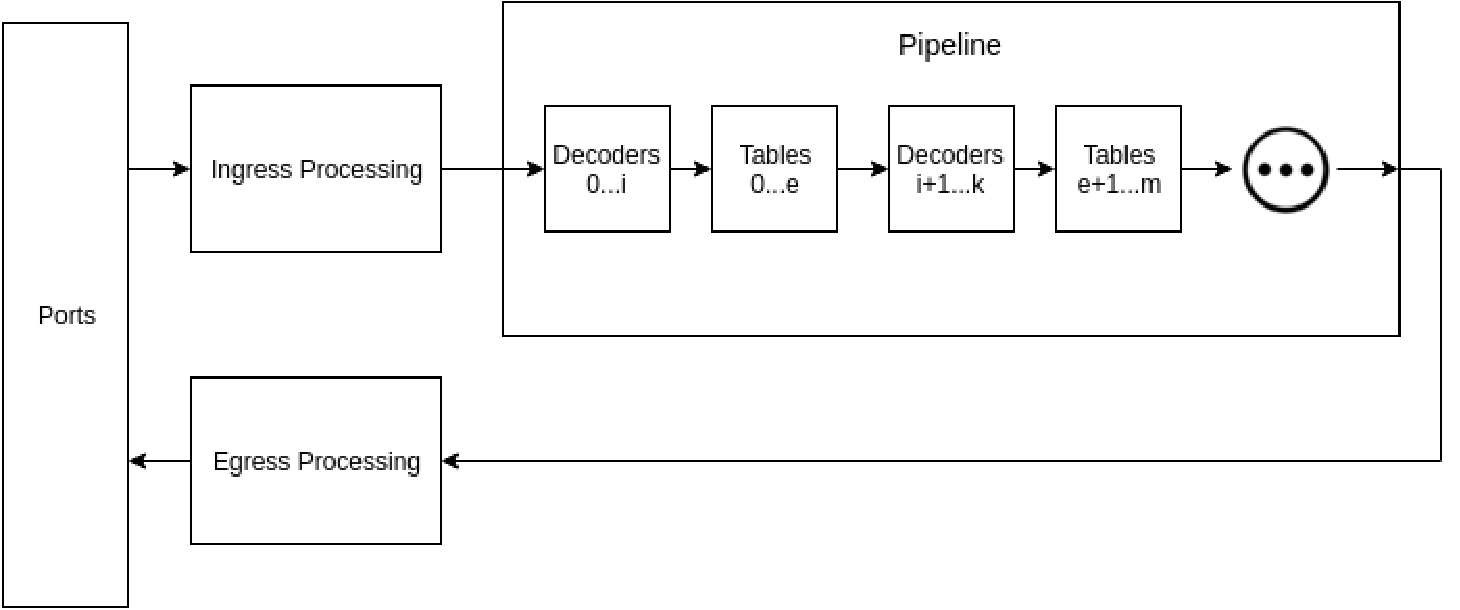
\includegraphics[width=\textwidth]{pipeline}
\caption{Packets entering the device go through ingress processing.
Then a pipeline composed of decoders and tables decide where the packet
should be forwarded. Once the decision is made, the packet goes through
egress processing before being forwarded.} 
\label{fg:pipeline_model} 
\end{figure}

The Steve pipeline can be described in terms of three phases: 
1) ingress processing, 2) pipeline processing, and 3) egress processing. 
The pipeline processing phase can be further decomposed into two kinds
of stages: decoders and flow tables.

%The Steve pipeline processing model can be described in terms of four phases: 1)
%\emph{ingress processing}, 2) \emph{decoding stages}, 3) \emph{table
%matching stages}, and 4) \emph{egress processing}. Figure
%\ref{fg:pipeline_model} depicts this pipeline processing model. One must
%understand this model to be able to write a Steve pipeline application.


\subsection{Ingress Processing} \label{ingress_desc}

Ingress processing is the the first phase every packet will go through.
A packet enters a network device on a port, known as its \emph{ingress port}.
At this time, the data plane builds a data structure known as the
\emph{context} around the packet. 
Contexts save additional data about a packet as it moves through the pipeline.
They serve as the input and output between pipeline stages.
Further explanation of the context can be found in Section \ref{context_desc}.

After ingress processing, the data plane dispatches the context (which includes
the packet) to the first decoding stage. The ingress processing stage is not
something that is written in a Steve application. It is implicitly handled by
the runtime system which manages data plane resources described in Chapter
\ref{ch:flowpath}.

\subsection{Contexts} \label{context_desc}

A \emph{context} is a data structure used to save and carry
additional metadata and stateful information about a packet between pipeline stages.
Pipeline stages may use this data structure to memoize things they have learned
about a packet. Specifically, the context data structure contains:

\begin{itemize} 
\item The packet itself. From now on, anytime mention of the
context is made, it is implied that this also includes the packet. 

\item
The packet's logical and physical ingress ports. 

\item The egress port. This
field is written to during pipeline processing. It ultimately determines which
port the packet gets forwarded on. 

\item The packet's length. 

\item A tunnel identifier used for handling virtual networks.

\item A \emph{binding environment} used to memoize the offset
and length of header fields. 

\item A \emph{binding environment} used to memoize the offset
of protocol headers. 

\item An \emph{action list} that may be written to and is
executed during egress processing. 
\end{itemize}

The two important data structures contained within a context are 
the \emph{action list} and the \emph{binding environment}.
Actions, which are described in Section \ref{action_desc}, are appended
to the action list using a write action.
These actions are executed during egress processing in the 
order that they were appended.

A binding environment is a data structure which maps object names to
corresponding storage locations at runtime \cite{compilers1}.
The storage location of fields is represented using an \emph{(offset, length)} pair, where \textit{offset} is the absolute offset of the field.
These mappings are known as \emph{bindings}. Figure \ref{fg:context1} 
depicts the abstract structure of a binding environment while Figure \ref{fg:context2}
depicts the contents of a binding environment during the decoding of an IP-in-IP packet.

\begin{figure}[ht]
\begin{subfigure}[t]{.45\textwidth}
  \centering
  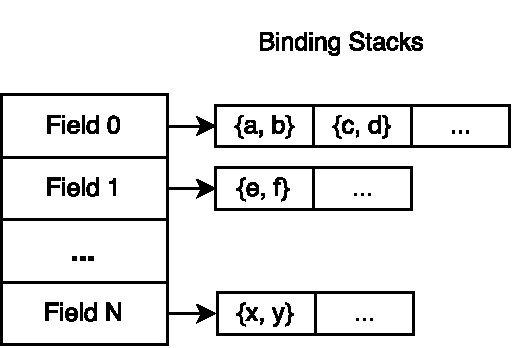
\includegraphics[width=\linewidth]{context}
  \caption{An abstract example of a binding environment.}
  \label{fg:context1}
\end{subfigure}
\hfill
\begin{subfigure}[t]{.45\textwidth}
  \centering
  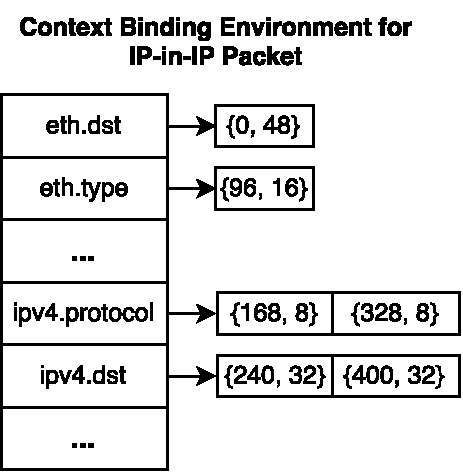
\includegraphics[width=\linewidth]{context_concrete}
  \caption{The contents of an environment when decoding an IP-in-IP packet. The header order in this example is Ethernet, IPv4, encapsulated IPv4, etc. Offset and length are given in bits (though implementations
  may choose to use bytes as the unit of measure).}
  \label{fg:context2}
\end{subfigure}


\caption{The Steve binding environment maps field names to stacks of
  \emph{(offset, length)} pairs. This allows multiple fields of the same
  name to be extracted and also supports fields being rebound with new names.}
\label{fg:ContextEnv}
\end{figure}

Since any given packet can contain one or more of any field or header with the
same name, a binding environment maintains a stack for every field and header.
These stacks are called \emph{binding stacks}. A binding environment is thus a 
mapping of field names to binding stacks. 
When the value of a field is needed, 
the topmost binding on the binding stack, i.e. the
most recently extracted field with that name, shall be used.

The field binding environment allows for the full memoization of all
extractions made during pipeline processing. It also allows fields to
be rebound with new names where necessary. It is of note that this
approach is heavyweight, that is, it is space consuming and may be
more information than is necessary for certain network functions.

%Figure \ref{fg:ContextEnvWorking} demonstrates how data is stored in the context
%as it is being decoded. The example is a packet which contains an encapsulated
%IPv4 header commonly used in IP tunneling. First, the ethernet \texttt{macdst}
%(mapped to index 0), \texttt{macsrc} (mapped to index 1), and \texttt{ethtype}
%(mapped to index 2) fields are extracted and stored in the context. Then the
%first IPv4 header's \texttt{ipdst} (mapped to index 3) and \texttt{iptype}
%(mapped to index 4) fields are extracted. After that, another IPv4 header's
%\texttt{ipdst} fields are extracted. If the value of
%\texttt{ipdst} is used in the program, it is the second one which gets used.
%
%\begin{figure}[ht]
%\begin{subfigure}[t]{.45\textwidth}
%  \centering
%  \includegraphics[width=.8\linewidth]{cxt_pkt_ex}
%  \caption{An example packet with ethernet, IPv4, and nested IPv4 header.}
%  \label{fg:view1}
%\end{subfigure}%
%\hfill
%\begin{subfigure}[t]{.45\textwidth}
%  \centering
%  \includegraphics[width=.8\linewidth]{cxt_s1}
%  \caption{Binding the fields in the ethernet header.}
%  \label{fg:view2}
%\end{subfigure}
%
%\begin{subfigure}[t]{.45\textwidth}
%  \centering
%  \includegraphics[width=.8\linewidth]{cxt_s2}
%  \caption{Binding fields from the first IPv4 header.}
%  \label{fg:view3}
%\end{subfigure}%
%\hfill
%\begin{subfigure}[t]{.45\textwidth}
%  \centering
%  \includegraphics[width=.8\linewidth]{cxt_s3}
%  \caption{Binding fields from the second IPv4 header.}
%  \label{fg:view4}
%\end{subfigure}
%\caption{A context environment in
%action during runtime.} \label{fg:ContextEnvWorking} 
%\end{figure}
%
%The \emph{action list} is the other major data structure contained within the
%context. An action list in Steve is a sequence of \emph{actions}. Actions are
%written to the action list for \emph{deferred execution}
%through the course of pipeline processing. These actions are executed in the
%order with which they were written once the
%packet completes pipeline processing, during the egress processing phase.

\subsection{Decoder Stages} \label{decoder_desc}

A packet is a chunk of raw uninterpreted binary data.
In order to make meaningful decisions, the program needs to
recover protocol headers whose fields contain the control
information needed to forward the packet.
Decoders are responsible for determining which
groups of bits are a header, and which subsets of that header form fields. 
The decoder then extracts those fields for usage by later stages.
Since a packet is composed of a sequence of headers, those headers and fields
may be extracted by a series of decoders linked together in a Steve pipeline.

A decoder operates on exactly one header.
It knows where fields are in that header by conforming to a header \emph{layout}.
Layouts allow Steve programmers to specify the structure of a
protocol header: what fields it contains, the length of those
fields, and the order of those fields.
The layout used by a decoder is known as its \emph{layout rule}.

Extracted fields are stored as \emph{(offset, length)} pairs in
the context binding environment. 
This format of decoding was inspired by work done in Protocol-Oblivious Forwarding 
(POF) \cite{pof, pof_fis, pof_impl}.
However, Steve does not require the programmer to specify these pairs manually.
The pairs are compiler generated using information from a
decoder's layout rule.

\subsection{How Decoder's Safely Extract Fields} \label{tut:extract_how}

Steve ensures that decoders have constrained
access to a subset of contiguous bytes in a packet buffer.
This is known as a decoder's \emph{view} of the packet.

A decoder's view begins where the header it decodes begins, and ends
(implicitly) where that header ends. 
This constrained region is enforced by the decoder's layout rule. 
That is, a decoder only knows about bytes up to and including the final field given in a layout and cannot know about or access any fields past that point.

A packet's context maintains the beginning of the current view using
a \emph{view index}. Once a decoder is finished executing, it is
responsible for shifting this view index so that it refers to the
first byte of the next header.

Figure \ref{fg:decoding} demonstrates how decoders extract fields and
how this view mechanism is applied on an actual packet instance. 
Here, the Steve application decodes a typical packet 
containing ethernet, IPv4, and UDP headers.

\begin{figure}[ht]
\begin{subfigure}[t, scale=0.5]{.45\textwidth}
  \centering
  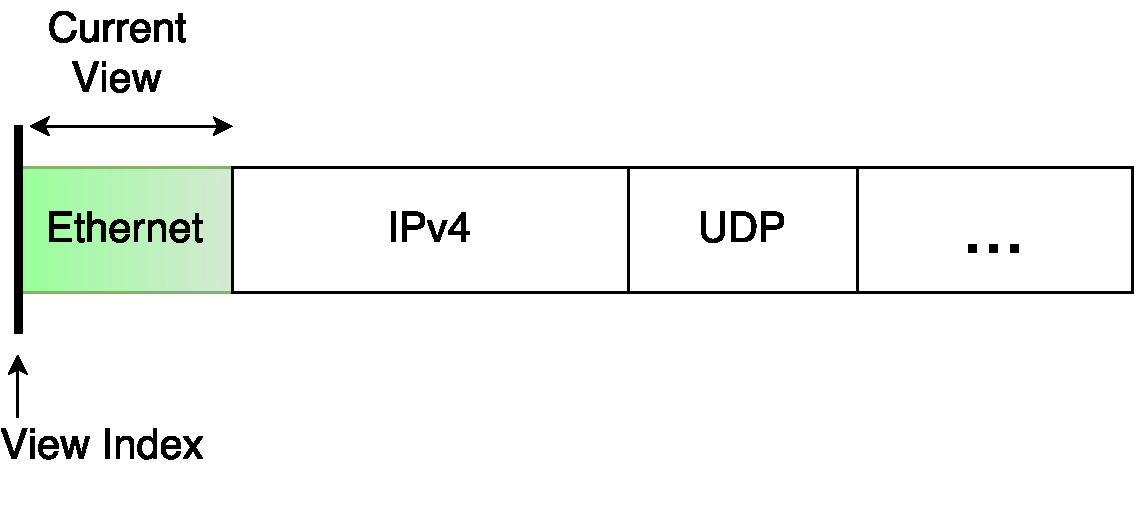
\includegraphics[width=\linewidth]{view1}
  \caption{The view of the first (Ethernet) decoder. 
  The beginning of the view is the beginning of the Ethernet
  header, which is also the beginning of the packet.}
  \label{fg:view1}
\end{subfigure}%
\hfill
\begin{subfigure}[t, scale=0.5]{0.45\textwidth}
  \centering
  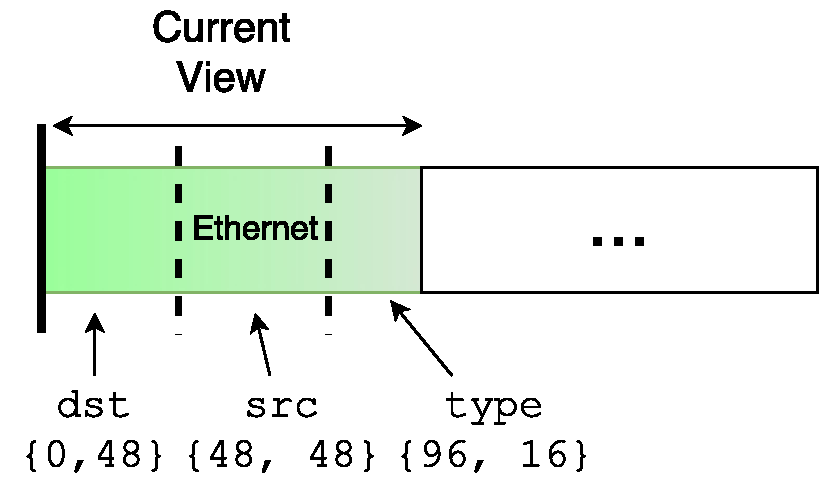
\includegraphics[width=.8\linewidth]{view2}
  \caption{The beginning of a field is discovered by its relative offset from
the beginning of the view. The end is determined by the field's length. The \texttt{dst} field has an offset of 0 and a length of 48 bits, 	\texttt{src} has an offset of 48 bits and a length of 48 bits, and \texttt{type} has an offset of 96 bits and a length of 16 bits.}
  \label{fg:view2}
\end{subfigure}

\begin{subfigure}[t]{.45\textwidth}
  \centering
  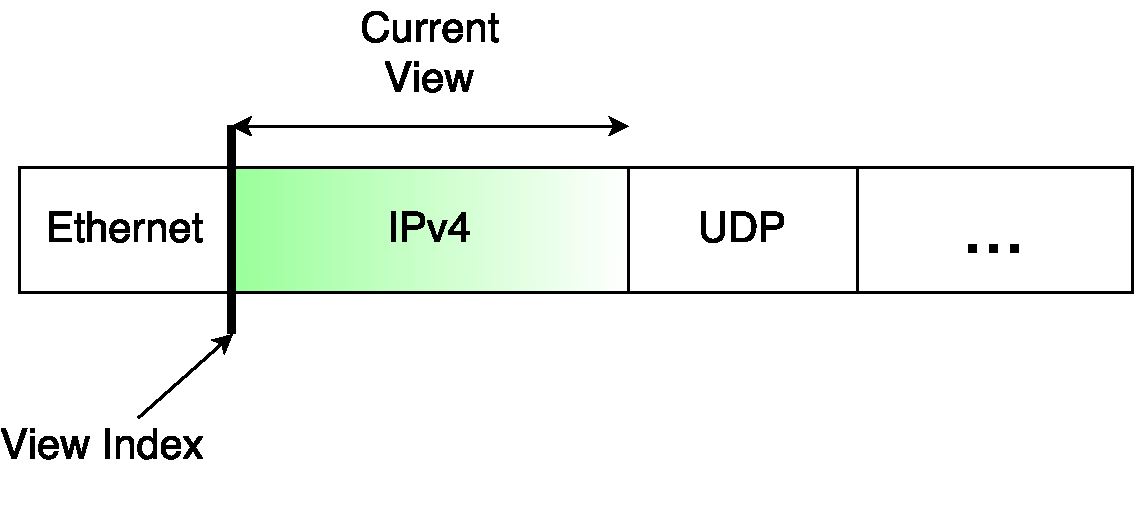
\includegraphics[width=\linewidth]{view3}
  \caption{When a decoder is finished working, it \textit{shifts} the view to
the next header. The shift moves the view index by the length of the current
header -- 14 bytes.}
  \label{fg:view3}
\end{subfigure}%
\caption{A demonstration of the decoding process in action.}
\label{fg:decoding}
\end{figure}

 
The view index always starts at the beginning of the packet.
In Figure \ref{fg:view1}, the first header is Ethernet.
In Figure \ref{fg:view2}, the three fields of the Ethernet header
are extracted.

When the compiler generates \textit{(offset, length)} pairs,
the \emph{offset} value is relative to the view index. The
absolute offset of the field is calculated using view index plus
the relative offset.
The absolute offset and length are saved in the context binding environment.
In Figure \ref{fg:view2}, the pairs \textit{(0, 48)} (\texttt{ethernet.dst}),
\textit{(48, 48)} (\texttt{ethernet.src}), and \textit{(96, 16)} 
(\texttt{ethernet.type}) are stored in the context.

%Each field in the header is discovered by information gathered by the layout
%rule. The layout rule tells a decoder the location, or relative offset, of
%each field from the beginning of the header (which is equivalent to the
%beginning of the view). It also gives the length of each
%field. From here, a decoder can go about discovering which bits form each
%field as demonstrated in Figure \ref{fg:view2}.

When a decoder finishes, it \textit{shifts} the view index, as seen in Figure
\ref{fg:view3}. The beginning of the view is moved by the length of header.
The view now starts one byte \textit{after} the previous header's final byte. 
All decoders are responsible for shifting the view in
preparation for the next decoder. Once the next decoder is reached, its view is
already on the header it decodes.

This process continues until all decoders are finished.
If at any point a layout is silently ill-defined 
(longer than the remaining packet memory), and a decoder tries
to extract a field which is past the bounds of the packet, the packet
is immediately dropped before the extraction completes.

\subsection{Partial and Full Decodes}

Steve provides full control over which fields get decoded
from a header. The entire header does not have to be decoded.
Steve allows for the extraction of only a subset of fields from a header. 
This is known as a \emph{partial decode}.
In some packet processing languages like P4 \cite{p4_spec, p4_spec2}, all
relevant headers have all their fields extracted before any pipeline processing
is done. 
This is known as a \emph{full decode}.
The issue is that full decodes are inherently wasteful.
Only certain fields and headers within a packet are ever really needed for a
forwarding decision.
Extracting any other fields is a waste of valuable processing time.
Due to the way Steve memoizes extracted fields, it also wastes space.
Efficiency is important when trying
to achieve software processing rates comparable to hardware line rate 
(10Gbps to 40 Gbps).

Not all headers need to be decoded either. For
example, if a networking application only needs to forward using MAC addresses,
there is no reason to waste time extracting fields from IPv4 or IPv6 headers,
and so on. It is up to the programmer to express how deep they wish to look into
a packet.

That being said, Steve supports the full decode as well. It may be desirable to
some programmers to do this in certain scenarios, thus the language does not
favor one paradigm over another.

\subsection{Table Stages} \label{table_desc}

Tables stages are used by the pipeline to make forwarding decisions.
A network \emph{flow} is a series of packets from a source to a set of one or
more destinations.
Table stages use the mechanism known as \emph{flow tables} to establish these
flows \cite{openflow_spec}. 
Flow tables are specialized decision tables which classify packets into
groups (flows) based on field values found in their headers. 
A common set of actions are then applied to classified packets.
Table \ref{tbl:flow_table} provides an example flow table.

\begin{table}[ht]
\caption{An example flow table matches on IPv4 destination and TCP protocol
destination port.}
\label{tbl:flow_table}
\centering
\begin{tabularx}{\linewidth}{| c | X | X | X |}
\hline
% Header of table
\multirow{2}{*}{Priority} & Key: IP Destination & Key: TCP Destination port  &
\multirow{2}{*}{Actions} \\
\cline{2-3}
  & \multicolumn{2}{|c|}{Match Fields} & \\
\hline
\hline
% beginning of flows.
1 & 10.1.1.0 & 80 & Set IP Dest. equal to 192.168.1.30. Output to port 1. \\
\hline
1 & 192.168.1.31 & 23 & Drop packet. \\
\hline
1 & 192.168.1.32 & 443 & Output port 2. \\
\hline
... & ... & ... & ... \\
\hline
\end{tabularx}
\end{table}


A flow table has a \emph{key} and a set of \emph{flow entries}. A
key specifies a set of fields from a packet, called \emph{key fields}, that a table matches
against (or classifies with). They are the equivalent of decision attributes.
Table \ref{tbl:flow_table} has two key fields: IP destination and TCP
destination port.

A flow entry is equivalent to a rule in a decision table. Each flow entry is
composed of \emph{match fields}, a \emph{priority}, a set of
\emph{actions}, and miscellaneous additional metadata (called
\emph{properties}). Table \ref{tbl:flow_table} has three sample flow entries
(with properties omitted).

For each key field, each flow entry has a corresponding value for that
key field, known as a
\emph{match field}. Each flow entry in the table must be uniquely
identifiable by its match fields and its priority.
Priority is an extra field used to
unambiguously execute exactly one flow entry if a packet matches
multiple flow entries.
The highest priority flow entry is always executed.
In this example, the first flow entry's match fields are
10.10.1.0 (IP destination) and 80 (TCP port destination), and its priority is 1.

When a packet is being matched
against a table, the fields given by the table's key are extracted from the
context. These extracted fields, together, are called the \emph{packet} or \emph{query key}.
Each match field is then compared against the corresponding packet field.
If all fields match, then the flow entry's actions are executed on the packet.
Actions may modify the packet, context, or flow tables and are discussed in Section
\ref{action_desc}.
In this example, if a packet with an IP destination of 10.10.1.0 and a TCP port
destination of 80 were matched against Table \ref{tbl:flow_table}, it would
match the first flow entry. It would have its IP destination changed to
192.168.1.30, then it would be forwarded to port 1.

If no flow entry matches the packet's field values, the \emph{miss case} flow
entry is applied to the packet instead. By default, a miss case will drop the
packet, but the behavior can be user defined. Miss cases always have the lowest
possible priority amongst flow entries and each match field can be considered a
wildcard.

The mechanic of table matching is also analogous to that of relational or SQL
tables (which coincidentally can be used to implement decision tables). In fact,
Frenetic, another SDN language, uses SQL-inspired syntax to
classify packets \cite{foster2011frenetic, foster2013frenetic}. In this comparison, a flow table is analogous to a relational table, the concept of a
key is the same for both, and a flow entry is analogous to a tuple in a SQL
table. Each packet and its fields "queries" the table for flow entries with
matching keys.

\subsection{Actions} \label{action_desc}

Actions may modify a packet, forward it, move it to a new stage, or modify a
flow table. 
Actions are primarily applied by flow tables, but may also appear in decoders
and event handlers.

\begin{itemize}

\item \textbf{Output}. This is used to forward a packet to a designated port.

\item \textbf{Drop}. This forces a device to drop a packet and delete its context.

\item \textbf{Decode}. This action is a \emph{transition action}. It sends the
packet from the current stage to another decoder.

\item \textbf{Goto}. This action transitions a packet from the current stage
to another flow table matching stage.

\item \textbf{Raise}. This action sends a copy of a packet and context to
be executed by an event handler. 
The original packet continues through pipeline processing as usual.

\item \textbf{Insert flow entry}. This inserts a flow entry into
a given flow table.
Inserting a flow entry that already exists will
remove the old one and replace it with the new one. 

\item \textbf{Remove flow entry}. This removes a flow entry from a flow table.
If the entry does not exist, nothing is done.

\item \textbf{Set.} This is used to modify a field in the packet.

\item \textbf{Write.} Write action allows actions to be appended to the context's
action list. Only set and output actions may be written.

\item \textbf{Clear.} The clear action removes all actions from the action list.

\end{itemize}

\subsection{Pipeline Execution}

Steve pipeline programs follow a run-to-complete model of execution. Once a
packet enters the pipeline, each stage is consecutively applied to
the packet. Once no more stages are applied, the packet exits the pipeline and
the next packet enters.

\subsection{Pipeline Composition} \label{pipeline_comp_desc}

Kinds of processing stages can be interleaved together in any order within the
pipeline unlike other languages like P4 \cite{p42014, p4_spec}. 
Upon entering the pipeline, a packet must first go through at least one decoding
stage before moving to the next processing stage. After that, there are many
possibilities.
Steve pipelines allow a user to specify the following pipeline compositions.

\begin{enumerate} 
\item \textbf{A complete decode of the packet followed by a
sequence of tables.} Packets have all necessary headers and fields decoded and
saved in the context first. The packet is then dispatched to the first table in
the pipeline which will send it to more tables until a forwarding decision is made.
Figure \ref{fg:pipeline1} depicts this pipeline.

\item \textbf{A chain of partial decodes and table lookups.} Packets get
partially decoded and dispatched to a table. The flow entry could carry the
packet to another table, another decoder, or forward it out of the network. The
pipeline is thus a chain of alternating sequences of decoding stages and table
matching stages. 
Figure \ref{fg:pipeline2} depicts this pipeline.

\item \textbf{Only decodes.} In some extreme cases, it may not
even be necessary to go to a table matching stage. It may be possible to make a
decision about a packet’s ultimate destination immediately upon evaluating a
certain field within the packet using a simple conditional statement
(if-statement, etc).
\end{enumerate}

\begin{figure}[ht]
\begin{subfigure}[t]{\linewidth}
  \centering
  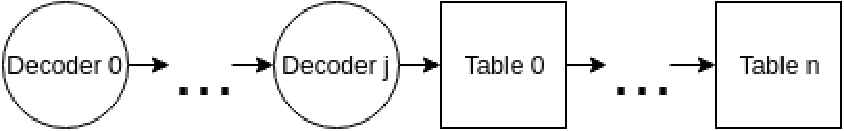
\includegraphics[scale=0.65]{pipeline1}
  \caption{A pipeline composed of a series of decoders followed by a series
  of tables.}
  \label{fg:pipeline1}
\end{subfigure}
\hfill
\begin{subfigure}[t]{0.95\linewidth}
  \centering
  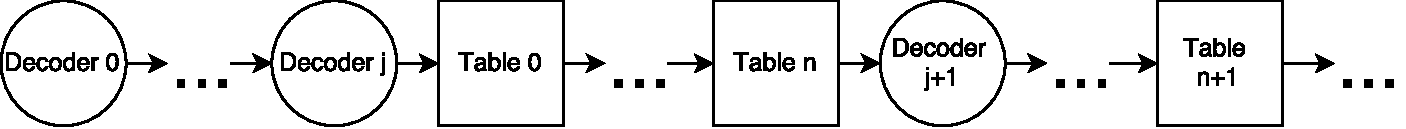
\includegraphics[width=0.95\linewidth]{pipeline2}
  \caption{A pipeline composed of alternating series of decoders and pipelines.}
  \label{fg:pipeline2}
\end{subfigure}

\caption{Kinds of pipeline composition.}
\label{fg:ContextEnv}
\end{figure}

\subsection{Egress Processing} \label{egress_desc}

Pipeline processing completes when a pipeline stage has finished executing
without sending the packet to a new stage. At this point the packet leaves the
pipeline and enters egress processing.

First, all actions written the context's action list are executed. Then the data
plane will check the egress port field in the context. If this has been set,
then the data plane will queue the packet up to be forwarded through that port.
Otherwise, the packet is dropped. The context is then destroyed.

\section{Event Handling} \label{events_desc}

Event handlers serve as hooks into the switch's control plane. 
As depicted in Figure \ref{fg:abstract_switch}, when a pipeline
cannot deal with a packet, it raises an event which is 
handled by an event handler executed in the control plane.
This event handler takes a copy of the context which raised the
event as an argument and performs some processing.
Event handlers may then choose to make calls back into the data plane's
pipeline to modify its behavior to accommodate for future packets.

An event is not guaranteed to execute in the typical run-to-complete model.
It is designed to be executed asynchronously by the runtime environment.
Certain slower operations which can
bottleneck the run-to-completion pipeline are typically performed in event
stages. This can involve inserting and removing flow entries to change the
pipeline, logging through use of C library functions, etc.

\section{Steve Compilation} \label{compile_desc}

Steve compiles into LLVM IR which is then optimized and compiled
again into a dynamic link library (DLL).
This DLL is loaded by the
Freeflow runtime environment described in Chapter \ref{ch:flowpath}.
Steve programs the Freeflow pipeline and acts as its software control
plane.